\chapter{Images}
\label{images}

\begin{figure}
    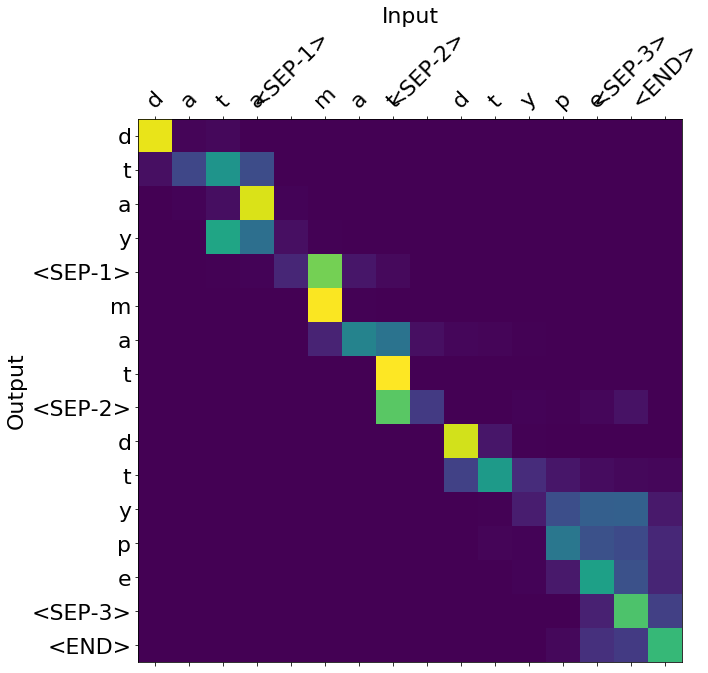
\includegraphics[width=0.8\linewidth]{images/typical_attention.png}
\end{figure}

\begin{table}
\begin{center}

\begin{tabular}{ | c || c |}
    \hline
    \hline
    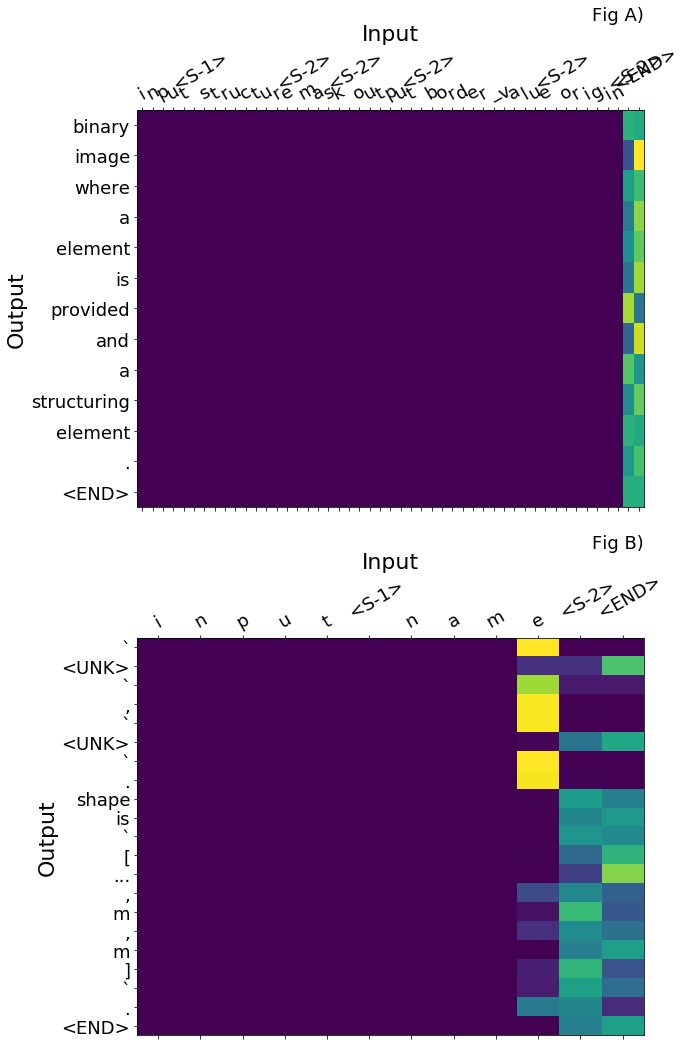
\includegraphics[width=0.5\linewidth]{images/otherargs_example.png}
    &
    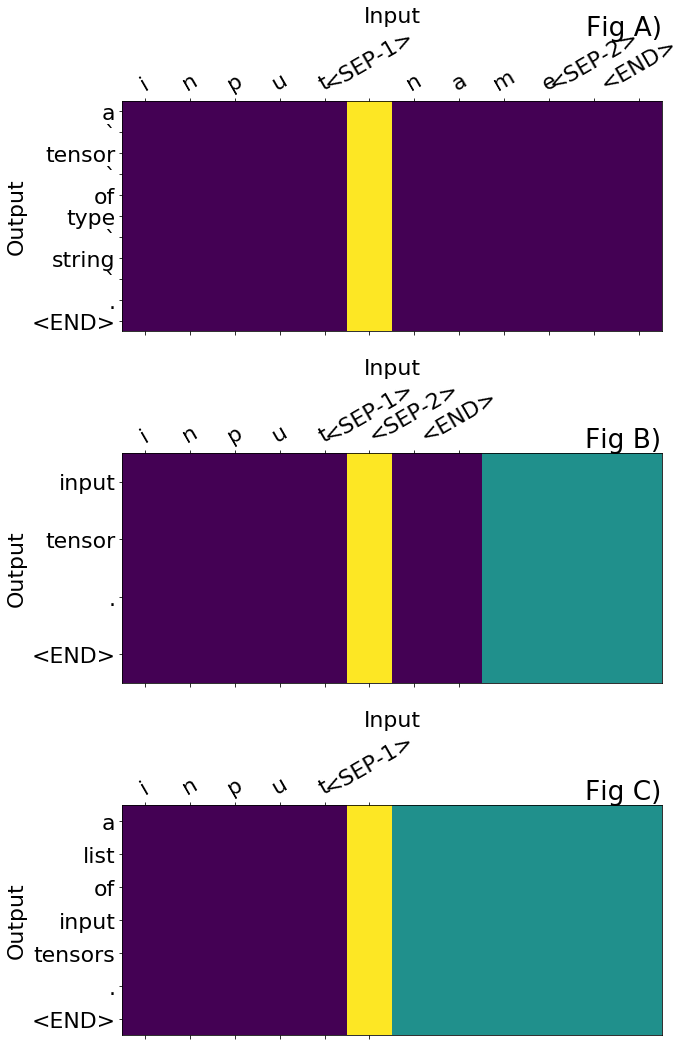
\includegraphics[width=0.5\linewidth]{images/different_translations_dupsXotherargs_3230minib.png} \\


    \hline

    \hline
\end{tabular}
\end{center}
\end{table}



\begin{table}
\begin{center}
\begin{tabular}{ l  }

\textbf{Nonsense}\\

\textbf{Input}: \textit{i n p u t $<$SEP-1$>$ s t r u c t u r e $<$SEP-2$>$ m a s k $<$SEP-2$>$ o u t p}...\\
...\textit{u t $<$SEP-2$>$ b o r d e r \_ v a l u e $<$SEP-2$>$ o r i g i n $<$SEP-2$>$ $<$END$>$}\\
\textbf{Description}: binary image to be propagated inside ` mask ` .\\
\textbf{Prediction}: binary image where a element is provided and a structuring element . \\

\\\hline\\


\textbf{Overfitting}\\

\textbf{I}: \textit{e n c o d i n g \_ t y p e $<$SEP-1$>$ s e l f $<$SEP-2$>$ d o c u m e}...\\
...\textit{n t $<$SEP-2$>$ r e t r y $<$SEP-2$>$ t i m e o u t $<$SEP-2$>$ $<$END$>$}\\
\textbf{D}: the encoding type used by the api to calculate offsets .\\
\textbf{P}: the encoding type used by the api to calculate sentence offsets . \\
\\\hline\\

\textbf{Underdetermination}\\

\textbf{I}: \textit{i n p u t $<$SEP-1$>$ n a m e $<$SEP-2$>$ $<$END$>$}\\
\textbf{D}: a ` tensor ` of type ` complex64 ` . a complex64 tensor .\\
\textbf{P}: ` $<$UNK$>$ ` , ` $<$UNK$>$ ` . shape is ` [ ... , m , m ] ` . \\
\\\hline\\
\end{tabular}

\caption{Three examples of typical errors in the character Seq-to-Seq model.  In this case, the first example shows good use of data in the sequence but is nonsensical. The second is an example of overfitting where the predicted sentence is found in the dataset. The final case, multiple sequences such as these are found in the dataset, each with a different discription. Without looking at code, or function name (in this case) it is impossible to disambiguate and the model fails to make sense }
\end{center}
\end{table}

\begin{table}
\begin{center}
\begin{tabular}{l}

\hline
\textbf{Validation Example}\\

\textbf{Input}: \textit{i n p u t $<$SEP-1$>$ s t r u c t u r e $<$SEP-2$>$ m a s k $<$SEP-2$>$ o u t p}...\\
...\textit{u t $<$SEP-2$>$ b o r d e r \_ v a l u e $<$SEP-2$>$ o r i g i n $<$SEP-2$>$ $<$END$>$}\\
\textbf{Description}: binary image to be propagated inside ` mask ` .\\
\textbf{Prediction}: binary image where a element is provided and a structuring element . \\

\\\hline


% \textbf{Training Example} in same function\\


% \textbf{I}: \textit{m a s k $<$SEP-1$>$ i n p u t $<$SEP-2$>$ s t r u c t u r e $<$SEP-2$>$ o u t p}...\\
% ...\textit{u t $<$SEP-2$>$ b o r d e r \_ v a l u e $<$SEP-2$>$ o r i g i n $<$SEP-2$>$ $<$END$>$}\\
% \textbf{D}: binary mask defining the region into which ` input ` is allowed to propagate .\\



% \\
% \hdashline
\textbf{Training Examples} starting $input$$<$SEP-1$>$$structure$\\
\\
\textbf{I}: \textit{i n p u t $<$SEP-1$>$ s t r u c t u r e 1 $<$SEP-2$>$ s t r u c t u r}...\\
...\textit{e 2 $<$SEP-2$>$ o u t p u t $<$SEP-2$>$ o r i g i n 1 $<$SEP-2$>$ o r i g i n 2 $<$SEP-2$>$ $<$END$>$}\\
\textbf{D}: binary image where a pattern is to be detected .\\
\\
\textbf{I}: \textit{i n p u t $<$SEP-1$>$ s t r u c t u r e $<$SEP-2$>$ i t e r a t i o n}...\\
...\textit{s $<$SEP-2$>$ o u t p u t $<$SEP-2$>$ o r i g i n $<$SEP-2$>$ m a s k $<$SEP-2$>$ b o r d e r \_ v a l u e $<$SEP-2$>$ b r u t e \_ f o r c e $<$SEP-2$>$ $<$END$>$}\\
\textbf{D}: binary array\_like to be closed . non-zero ( true ) elements form the subset to be closed .\\
\\
\textbf{I}: \textit{i n p u t $<$SEP-1$>$ s t r u c t u r e $<$SEP-2$>$ o u t p u t $<$SEP-2$>$ o r}...\\
...\textit{i g i n $<$SEP-2$>$ $<$END$>$}\\
\textbf{D}: n-dimensional binary array with holes to be filled\\
\\
\textbf{I}: \textit{i n p u t $<$SEP-1$>$ s t r u c t u r e $<$SEP-2$>$ o u t p u t $<$SEP-2$>$ $<$END$>$}\\
\textbf{D}: an array-like object to be labeled . any non-zero values in ` input ` are counted as features and zero values are considered the background .\\
\\
\textbf{I}: \textit{i n p u t $<$SEP-1$>$ s t r u c t u r e $<$SEP-2$>$ i t e r a t i o n}...\\
...\textit{s $<$SEP-2$>$ m a s k $<$SEP-2$>$ o u t p u t $<$SEP-2$>$ b o r d e r \_ v a l u e $<$SEP-2$>$ o r i g i n $<$SEP-2$>$ b r u t e \_ f o r c e $<$SEP-2$>$ $<$END$>$}\\
\textbf{D}: binary image to be eroded . non-zero ( true ) elements form the subset to be eroded .\\
\\
\textbf{I}: \textit{i n p u t $<$SEP-1$>$ s t r u c t u r e $<$SEP-2$>$ i t e r a t i o n}...\\
...\textit{s $<$SEP-2$>$ m a s k $<$SEP-2$>$ o u t p u t $<$SEP-2$>$ b o r d e r \_ v a l u e $<$SEP-2$>$ o r i g i n $<$SEP-2$>$ b r u t e \_ f o r c e $<$SEP-2$>$ $<$END$>$}\\
\textbf{D}: binary array\_like to be dilated . non-zero ( true ) elements form the subset to be dilated .\\
\\



\end{tabular}

\caption{A validation example and the a selection of training points. Despite being a long sequence, }
\end{center}
\end{table}

